\section{Implementation choices}
In this section we describe the proposed architecture in more detail. We present the excerpt on the internal structure of both public and private chains and the reasoning behind these choices.

In order to deduce the internal structure of our system, we will first analyze its use-cases. The overview of the education process is given in section \ref{sec:architecture}. The communication between the Student and the Educator is saved as transactions in the private chain. However, the implementation details of this chain mostly depend on the data disclosure process.

We will start from analyzing this process and determining the main issues that arise from the need to disclose and verify the validity of the private blocks. Then we will propose the structure of the private and public blocks that addresses these issues.

\subsection{Anonymity and certification}
\label{sec:cert}
The permissionless nature of our public chain leads to the ability for malevolent students to create educational institutes in order to get the scores for the courses they did not attend. Moreover, the knowledge students actually get by completing the course, and the conditions upon which the course is considered completed, vary significantly between the educational institutions. 

These issues currently can not be solved solely on the protocol level: they require an external source of information to determine the physical existence and the reputation of an Educator. Although we leave the public chain open for the Educators to submit their private block headers, we propose to add a separate layer of reputation and trust on top of the protocol.

We do so by introducing the Archivists -- the entities that join the network with the approval from another Archivist. Their main role is to add a trust level above just the raw protocol: they store the certificates of the Educational institutes and have the right to revoke those certificates. Furthermore, the Archivists are the entities responsible for determining the ratings of the particular Educators. The Archivists base their rating on the off-chain sources of information and gain authority for providing valid ratings and performing all the necessary compliance procedures for the Educators.

While in theory the Recruiters can query the Educators directly and initiate a data disclosure request, they are generally discouraged to do so. We expect the Recruiters to be willing to pay extra fees to the Archivists for certificate validation and ranking of the Students depending on the Educators' ratings and other factors upon request. We describe the data disclosure process in detail in section \ref{sec:DataDisclosure}

\subsection{Activity Type Graph}
\label{sec:ATG}
When a Recruiter makes a request to one of the Archivists, the Archivist has to somehow choose the relevant Educators. Moreover, when an Educator discloses the data, it has to provide as minimal set of entries as possible. This set has to be verifiable, which means that the Educator provides the proof of the data validity along with the data being disclosed.

In order to achieve these goals, we divide the data that the Educators store into atomic Activity Types. Each Educator maintains a journal of transactions per each Activity Type that the Educator offers.

All the Activity Types are grouped into courses that are further grouped into larger entities such as subjects and areas of knowledge. This grouping can be stored as the Activity Type Graph $G_A$ with the following properties:
\begin{enumerate}[label=\arabic*${}^\circ$]
\item $G_A$ is a directed graph:
  \begin{equation}
  G_A:\ \langle V: \{\mathrm{Vert}\},\ e_{out}: \mathrm{Vert} \rightarrow \{\mathrm{Vert}\}\ |\ \mathrm{rest} \rangle
  \end{equation}

\item Each vertex of $G_A$ is associated with depth:
  \begin{equation}
  G_A:\ \langle d: \mathrm{Vert} \rightarrow \mathrm{Int}\ |\ \mathrm{rest}  \rangle
  \end{equation}

\item Law of pointing down:
  \begin{equation}
  G_A:\ \langle v \in e_{out}(u) \implies d(v) > d(u) \rangle
  \end{equation}

\item $G_A$ has special \textit{et cetera} vertices $u$:
  \begin{equation}
  \forall\ v \in V\ \exists u\ (u \in e_{out}(v) \land e_{out}(u) = \emptyset)
  \end{equation}
\end{enumerate}

The example of the Activity Type Graph (ATG) is shown in Figure \ref{fig:atg}. The vertex $v$ of the graph is a \textit{leaf} if $e_{out}(v) = \emptyset$. Otherwise we call it an \textit{internal vertex}. Every internal vertex of the graph has a special \textit{etc.} child (some of these are ommitted in the figure).

\begin{figure}[ht]
\centering
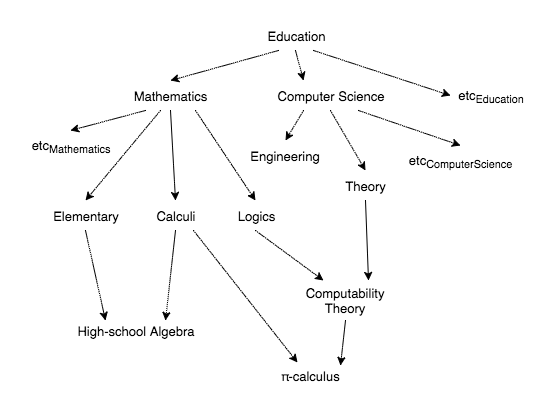
\includegraphics[width=0.8\textwidth]{atg}
\caption{An example of the Activity Type Graph. Some of the vertices are not shown}
\label{fig:atg}
\end{figure}

The need for \textit{etc.} vertices arises from the fact that not all of the Educators teach courses exactly in leaves — some of them offer general courses that provide just the necessary background. For example, some of the universities teach the basic \textquote{Computer science} course, that contains the basics of the discipline. In this case, when the particular category is hard to define, the university would use the $\textrm{etc}_{\textrm{ComputerScience}}$ vertex.

On the protocol level, the Educators can announce that they teach a particular course, but can not modify the Activity Type Graph structure. The structure of the graph is maintained by the core developers and updated upon request from the Educators.

\subsection{Private chain}

The structure of the private block is shown in Figure \ref{fig:privateblocks}. The block consists of a public \textit{header} that the Educators relay to the Witnesses, and the private \textit{body} that remains in the educational institute until it receives a data disclosure request.

\begin{figure}[ht]
\centering
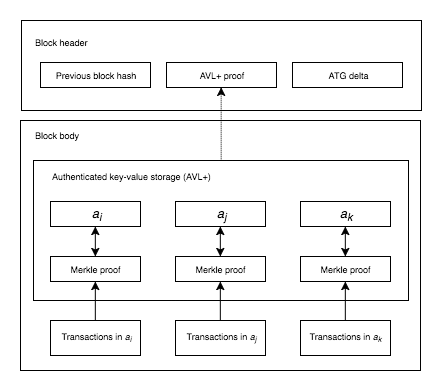
\includegraphics[width=0.8\textwidth]{private-blocks}
\caption{Private block structure}
\label{fig:privateblocks}
\end{figure}

During the educational process the Educators emit atomic \textit{private transactions}. These tansactions represent the modifications to the journal of academic achievements in a certain activity type (thus, making a transaction means appending the data to the journal of a particular course). The transactions can be of the following types:
\begin{itemize}
\item student enrolls in a course;
\item student gets an assignment;
\item student submits an assignment;
\item student gets a score for an assignment;
\item student gets a final score for the course.
\end{itemize}

Let us denote an $i$-th transaction belonging to a certain activity type $a_j$ as $T_{a_j}^i$. The Educators group the transactions that occured during the current block time slot according to the activity type, and construct Merkle trees \cite{merkle1989certified} for these journal modifications:
\begin{equation}
M_{a_j} = \textrm{MerkleTree}(T_{a_j}^i)
\end{equation}

The Educator's private block body contains a dictionary of key-value pairs, where each key is the leaf in the activity type graph $a_j$, and the values are the Merkle roots of all the transactions that occurred in this leaf in the current block. Thus, the private block body is a mapping:
\begin{equation}
a_j \rightarrow \textrm{root}(M_{a_j})
\end{equation}

In order to make this mapping easily verifiable, we use a structure called the \textit{authenticated AVL+ tree} introduced in \cite{reyzin2016improving}. This structure is based on state-of-the-art research that enables for faster verification of the mapping and allows us to never disclose it: the Witnesses would not have to store the whole blockchain like Bitcoin or Ethereum nodes do. Rather, they would just have to check the private block headers in order to confirm that none of the private blocks were tampered with.

The private block header consists of the AVL+ proof along with the previous block hash and the information on the Activity Type Graph modifications (ATG delta). The \textit{ATG delta} part allows the Educators to inform the Witnesses and the Archivists of the modifications to the courses they teach.

After the end of the block time slot, an Educator signs the block header and submits it to the Witnesses so that the private transactions can be confirmed by the public chain. Thus, the private blocks form a publicly verifiable chain of events, grouped according to the activity type.

\subsection{Public chain}
The Witnesses maintain a public chain -- a distributed ledger that contains publicly available information. If one wishes to perform a transaction on the public chain, she has to pay a certain fee that serves two purposes. First of all, the fee incentivizes the Witnesses to participate in the network and issue new blocks. Second, by requiring a fee for each transaction, we protect the public ledger from being spammed.

We present the structure of the public blocks in Figure \ref{fig:publicblocks}. The public ledger contains the following information:
\begin{enumerate}
\item Modification history of the Activity Type Graph.
\item Private transaction proofs.
\item Account balances and value transfer history.
\end{enumerate}

\begin{figure}[ht]
\centering
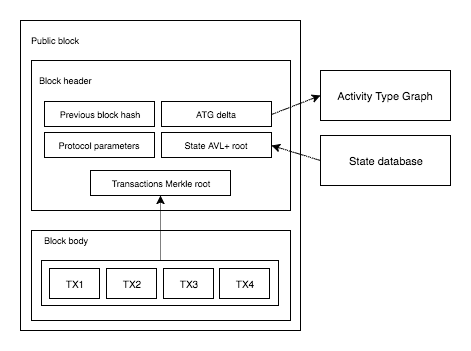
\includegraphics[width=0.8\textwidth]{public-blocks}
\caption{Public block structure}
\label{fig:publicblocks}
\end{figure}

There are two major ways to store the account balances and other state information: UTXO and account-based architectures. UTXO is an unspent transaction output, that contains some predicate -- a condition that has to be fulfilled in order to spend the coins. To prove the money ownership, the spender provides a witness -- an input that makes the predicate true. Thus, the UTXO-based architecture requires the transactions to be stateless, effectively limiting the application domain \cite{bentov2017instantaneous}.  The unspent outputs with an associated state can be treated as smart-contracts in the account-based architectures like Ethereum \cite{wood2014ethereum}. The state is stored in an off-chain storage -- the state database. The transactions are treated as the modifications of the world state. We are going to develop an UTXO-based ledger with transactions programmable in Plutus language \cite{Plutus}.

The recent achievements in the field of consensus protocols, like the provably secure Ouroboros \cite{kiayias2017ouroboros}, allow us to build a public chain based on the Proof of Stake consensus rules. Thus, we can increase the transaction speed and drop the need for the expensive mining. However, with mining being dropped, we need to provide incentives for the Witnesses to maintain the chain and participate in the network.

\subsection{Incentives}

In order to incentivize the Witnesses as well as the Archivists and the Object Store maintainers we propose a monetary policy with two main sources of income. The first one is the technical pool — a special pool of tokens, which are reserved until the participants acquire them through contributions to the operation of the platform. The tokens from the technical pool will be distributed with exponential slowdown. Running the nodes for different entities of the system require different hardware resources and there may come a point where the system lacks the nodes of a certain entity. To overcome this issue, the complexity and the amount of tokens received by the participants will be determined dynamically so that the equilibrium between the entities is preserved, for example, if the system lacks the Archivists, the incentive to run the Archivist's node would be more then the one for the Witnesses.

The second source of the participants' income is the fees for the transactions in the system. The Recruiters' fee is distributed among all the participants except the Object Store maintainers. The latter obtain tokens from the Educators paying them for the storage they offer.

\subsection{Fair CV}
One of the main goals of the Disciplina platform is to provide a way for the Students to easily prove their educational records. We propose to duplicate the records in the Student's \textit{digital CV.} This CV contains all the records that the parties have generated during the Student's educational process along with the validity proofs of that data (see figure \ref{fig:cv}).

\begin{figure}[ht]
\centering
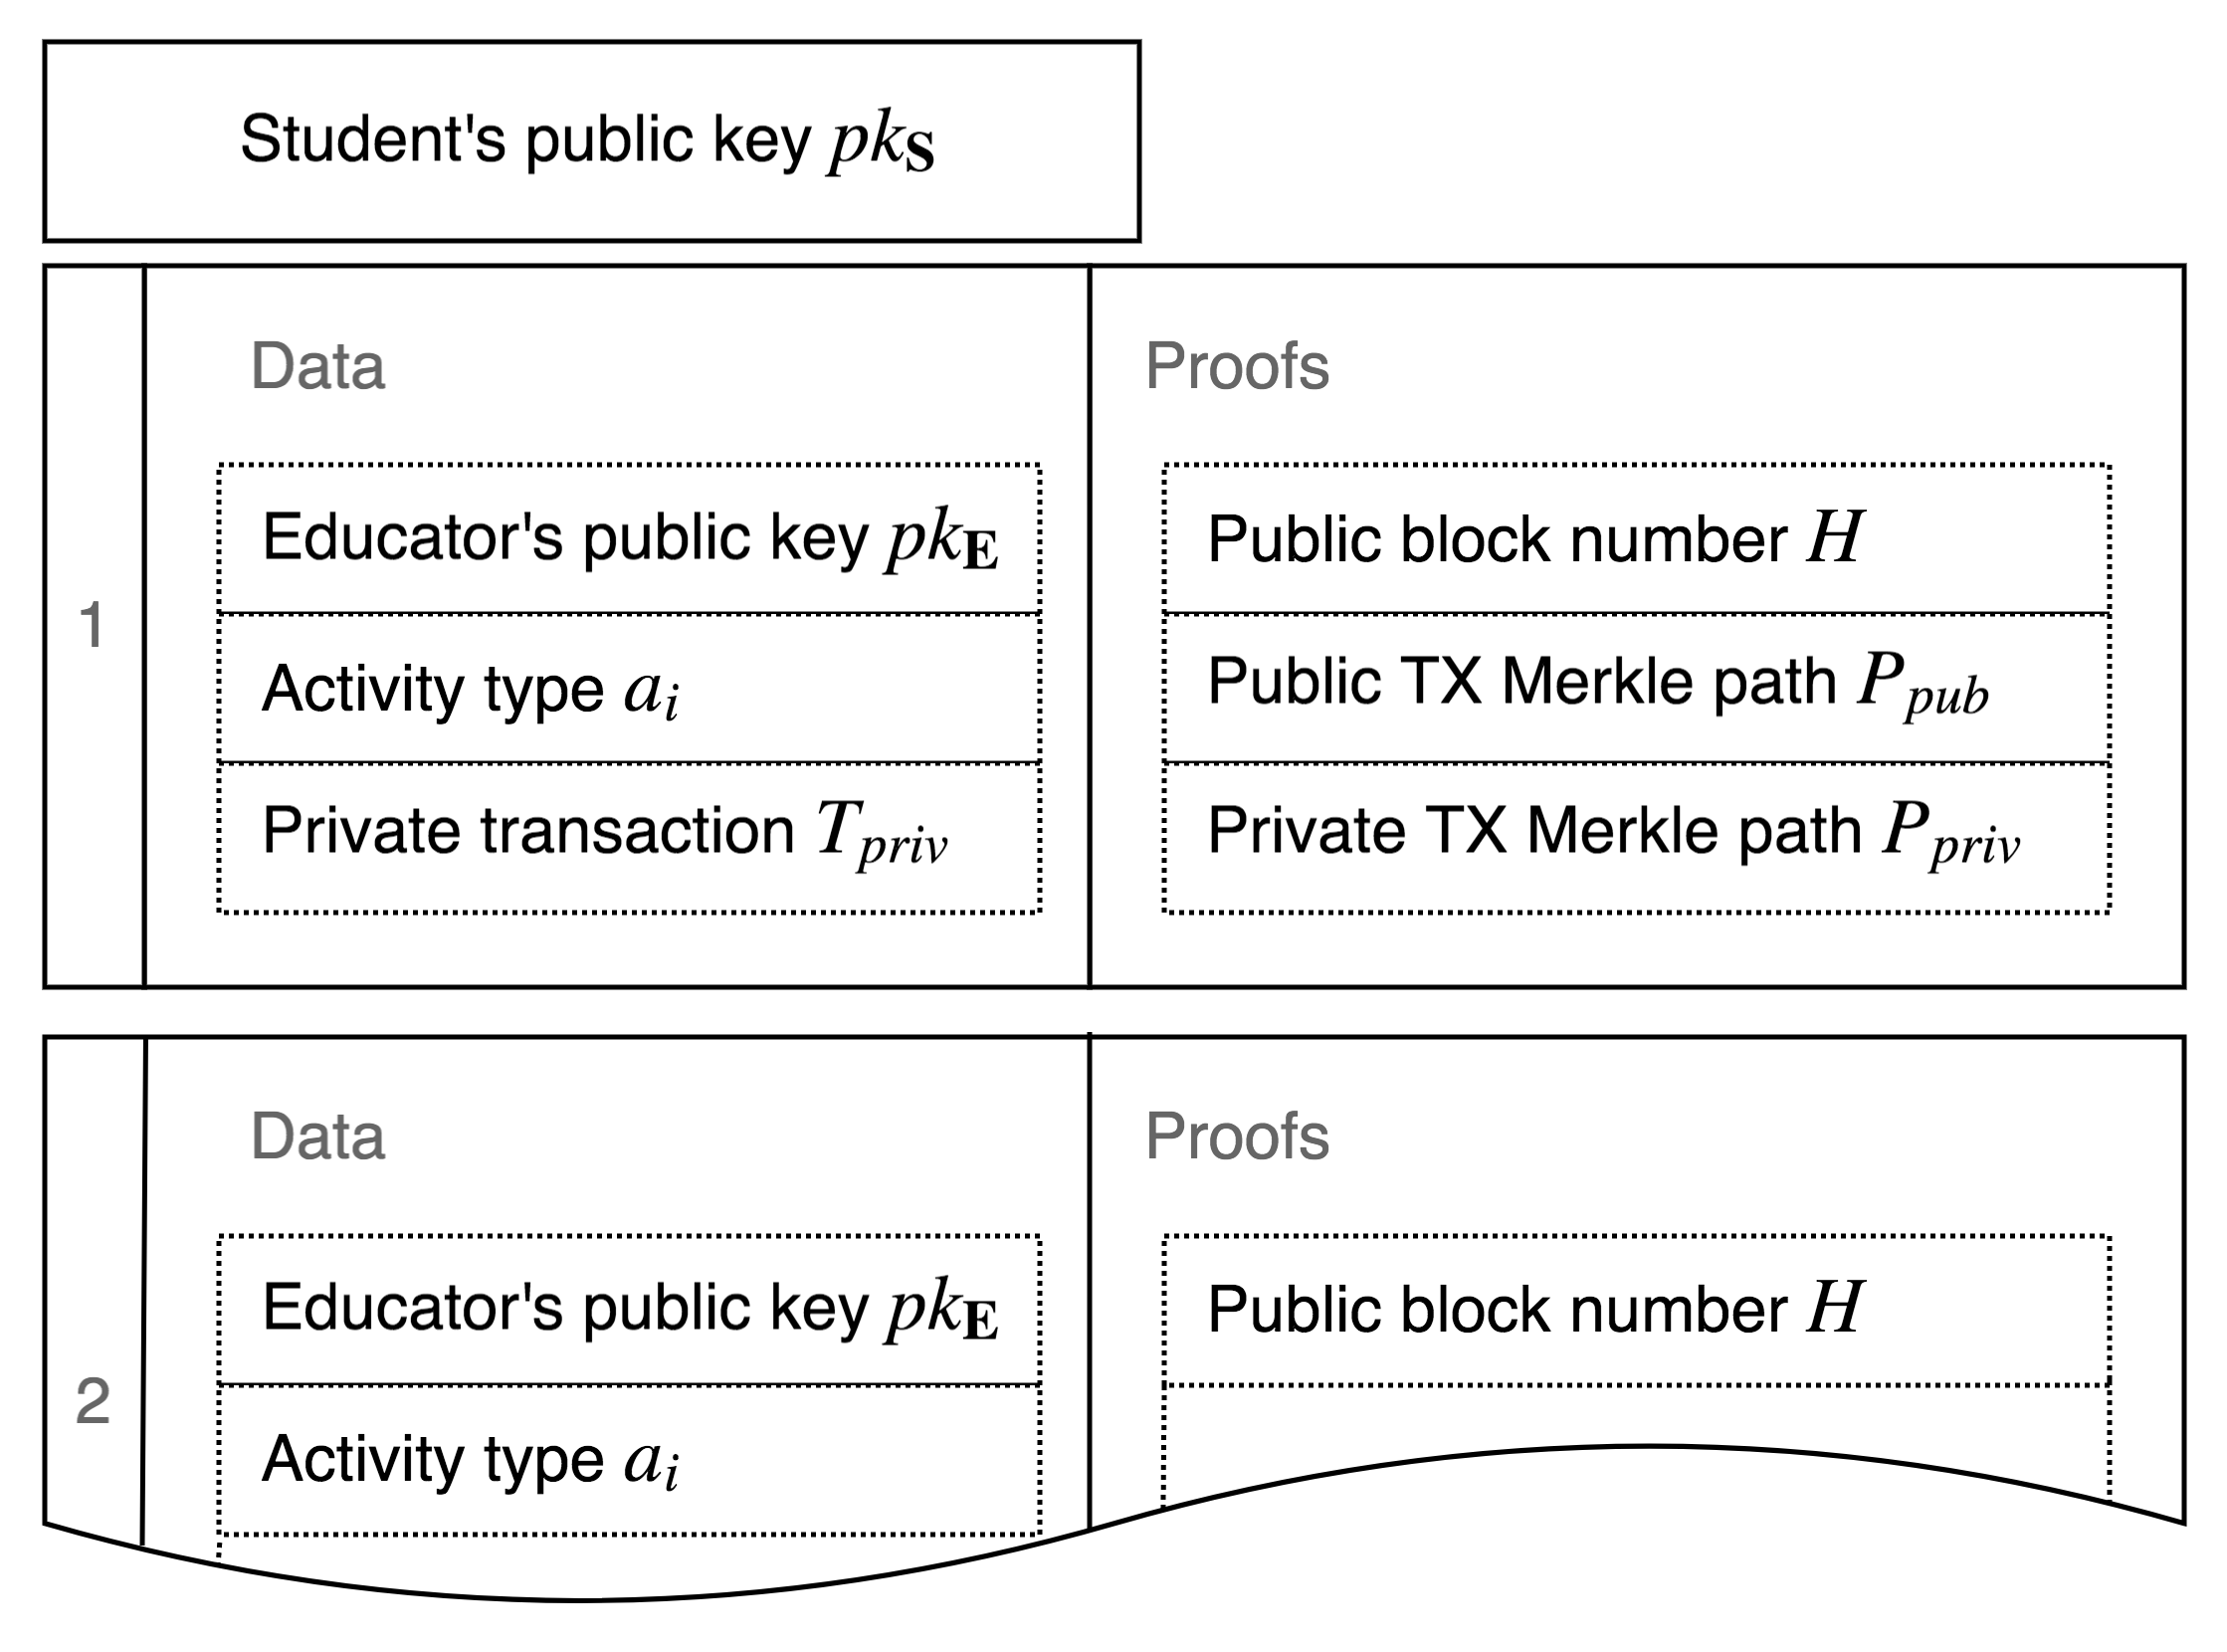
\includegraphics[width=0.8\textwidth]{cv}
\caption{Student's authenticated CV}
\label{fig:cv}
\end{figure}

In order to prove that the transaction actually occurred in some private block of a particular Educator, the student has to provide the cryptographic proofs along with the actual data. The cryptographic proof of the inclusion of an element in an authenticated data structure is generally a path of hashes. Let us denote the path of the element $e$ in the data structure $D$ as $\mathtt{path}(e, D)$. Thus, the Student has to  provide the following data:
\begin{itemize}
  \item The Student's and the Educator's public keys $PK_S$ and $PK_E$.
  \item The course $a_i$ and the a private transaction $T_{priv}$ with the score.
  \item The Merkle path of the transaction in the journal: $P_{M} = \mathtt{path}(T_{priv}, M_{a_i})$
  \item The AVL+ path to prove that the journal was included in a private block's AVL+ tree $A$: $P_{A} = \mathtt{path}(\mathtt{root}(M_{a_i}), A)$
  \item The public block number $H$ and the Merkle path of the transaction $T_{pub}$ that pushed the private block into the public chain: $P_{H} = \mathtt{path}(T_{pub}, M_H)$, where $M_H$ is a Merkle tree of the transactions in the block $H$.
\end{itemize}

Having this data one can prove the occurrence of a certain transaction in one of the Educator's private blocks without the need to request any data from the Educator during the validation process. Thus, any party can check the validity of the Student's CV for free if the Student wishes to disclose it.

Let $\rho(e, P)$ be the function that substitutes the element $e$ in path $P$ and computes the root hash of the authenticated data structure. Then the validation process is as follows:
\begin{enumerate}
\item Query the public chain to find the block $H$ and obtain the Merkle root of the transactions: $\mathtt{root}(M_H)$.
\item Check whether $\rho(T_{pub}, P_{H}) = \mathtt{root}(M_H)$.
\item Check that the public transaction $T_{pub}$ was signed with the Educator's public key $PK_E$.
\item From the public transaction $T_{pub}$ obtain the root of the AVL+ tree: $\mathtt{root}(A)$.
\item Use $PK_S$, $a_j$ and score to build a private transaction $T_{priv}$.
\item Compute $R_{M} = \rho(T_{priv}, P_{M})$.
\item Check that $\rho(R_{M}, P_{A}) = \mathtt{root}(A)$.
\end{enumerate}

These validation steps can prove that an Educator with a public key $PK_E$ issued a transaction $T_{priv}$ in one of its private blocks. One can attribute the $PK_E$ to a particular real-world educational institution by checking the Educator's certificate as described in section \ref{sec:cert}.

\subsection{Data Disclosure}
\label{sec:DataDisclosure}

The high-level data disclosure process is as follows:
\begin{enumerate}
\item Archivists keep records on all the Educators in the system along with the courses they teach.
\item The Recruiter sends data disclosure request to one of the Archivists.
\item The Archivist selects the relevant Educators and forwards the request.
\item The Educators determines the size of the data they are going to disclose.
\item Based on the size of the data, the Archivist informs the Recruiter of the cost of the request.
\item The Recruiter pays the fee.
\item The Educators send the data to the Archivist.
\item The Archivist checks the blocks received from the Educator for their validity using the data from the Witnesses' chain, and forwards this data to the Recruiter.
\item The fee is distributed between the relevant parties.
\end{enumerate}

The process of data disclosure involves direct communication between a particular Educator, willing to disclose a part of the data, and a Recruiter, willing to pay for this data. To mitigate the risk of secondary market creation, one should ensure that the majority of the data remains in the private blocks. Thus we reduce the size of the Educators' response by incentivizing the Recruiters to make as accurate requests as possible. We propose the following formula to determine the cost of the request:
\begin{equation}
\mathrm{Cost}(request) \sim \mathrm{exp}(N_{actions}(response))
\end{equation}

The value received from the Recruiter is then distributed between the Archivists, the Educators that disclosed the data, and the affected students.